In the previous section we explained why current cloud resource allocation approaches 
(see Figure~\ref{fig:static_allo}) 
are sub-optimal for HPC workloads. This section will introduce our proposed solution which combines 
CPU and memory over-commitment with virtualization for simultaneously achieving resource optimization and security isolation. Firstly, we start by introducing how to build multiple VCs with CPU over-commitment. Then, we continue to include and describe the more challenging memory over-commitment. Lastly, we analyze the 
potential pitfalls of resource over-commitment in a virtualized environment, 
and present dynamic VM migration as a mitigation to complete the whole picture.


%we complete the design 
%with dynamic VM migration, which mitigates potential 
%performance penalties from resource over-commitment. 

\subsection{CPU over-commitment}
With a share-based CPU scheduler in the hypervisor, the allocation of CPU resource among VMs on a host does not entirely rely on the number of vCPUs, but also is affected by the configurable CPU shares. 
This design change offers system admins the freedom to 
change VM vCPU count while maintaining the same resource allocation. We take advantage of this 
flexibility and configure each tenant with the same number of virtual CPUs as the physical cores 
on a node. In this way, each tenant can get access to all the cores inside the node, and consequently, if one tenant 
is not consuming its entire quota, the free CPU cycles can be used by other tenant(s). 
This approach can be easily scaled to a cluster by repeating the configuration on every 
single node. Then, each tenant is allocated a VC that consists of one VM per node. From the end user 
perspective, each tenant gets exclusive access to a dedicated cluster with isolation in security, fault, and even performance.  

Corresponding to a typical HPC cluster where there are login node(s), management node(s), 
and a set of compute nodes, the idea of CPU over-commitment can be illustrated in 
Figure~\ref{fig:architecture}. Every node is virtualized by running a hypervisor, 
such as VMware ESXi, in replacement of a conventional OS. On top of the hypervisor, 
a selected number of full-size VMs~\footnote{By full-size VM we mean the VM is configured with the same number of virtual CPUs as the physical cores.} 
can be configured on each node to over-commit the 
node's resources. Then, across the whole physical cluster, a VC
can be constructed by taking one VM per node and be allocated by system admins  
to a tenant. % with security isolation from other tenants. 
In this manner, each tenant will own his/her exclusive login, job scheduler, and worker VMs, thus ensuring full isolation from other tenants. 
Note that the actual physical 
CPU resources allocated to a VC, which largely determines the QoS guarantees, need to be 
carefully managed by the system admins by controlling the number of VCs sharing the physical cluster 
together with the relative CPU shares among the VCs.  

%Using the previous example of sharing four nodes between two tenants,  
%vHERO is illustrated in Figure~\ref{fig:vtc}. In the experiment section later, we will demonstrate  
%support of up to four tenants simultaneously on a single physical cluster with 4X CPU over-commitment.

\begin{figure}[!t]
   \begin{center}
       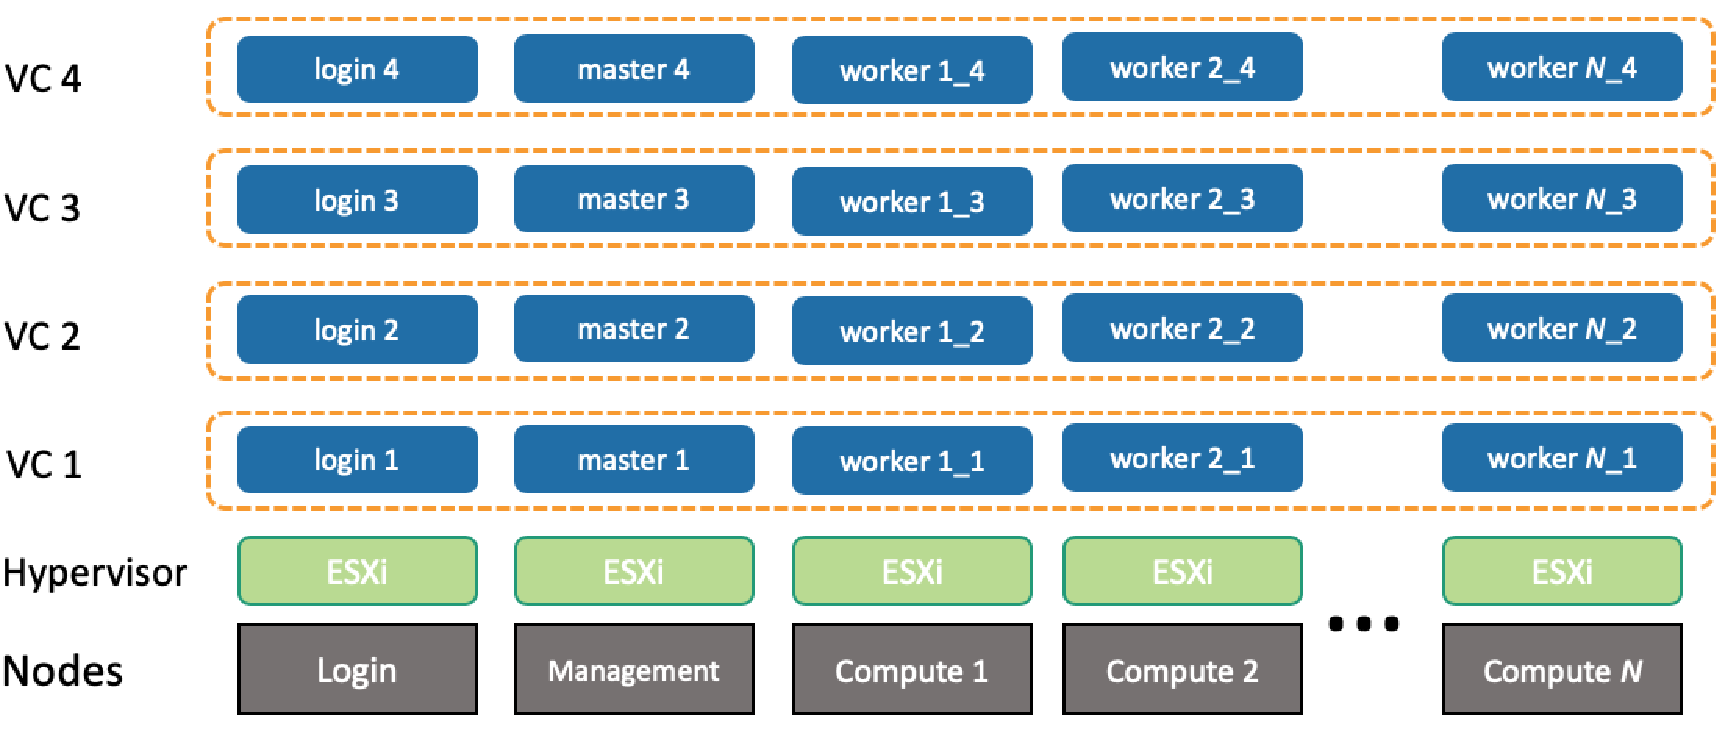
\includegraphics[width=\columnwidth]{Figures/architecture}
   \end{center}
   \caption{Illustration of four VCs with resource over-commitment. Each tenant can access a VC with dedicated login, job scheduler master, and worker VMs, with full isolation from other tenants.}
   \label{fig:architecture}
 \end{figure}

\subsection{Memory over-commitment}
Similar to CPU over-commitment, memory can be configured in a way that the total VM memory can be 
larger than the physical memory capacity. It is impractical, however, that all VMs actively access all configured 
memory beyond the physical capacity. This is mainly due to performance considerations. TPS, ballooning, and 
compression all have no guarantee to reclaim memory in a timely manner, and if all these techniques fall short, 
hypervisor swapping will occur to swap out guest OS memory to disk, rendering unacceptable performance to 
the HPC workloads. Three questions that we address in this paper through a combination of exploration and experiments are: 1) is there any way to mitigate 
memory reclamation impact while applying memory over-commitment; 
2) with mitigation, whether memory over-commitment 
can be practical for performance; 3) how far can we go with memory over-commitment.

\subsection{Dynamic VM migration}
It's very restricting that while one can configure more VM memory than the available physical capacity, the VMs are not able to consume all of it 
at the same time. This constraint applies to every node in the cluster because if memory is over stressed on any 
node, the progress of the whole workload is impacted. 
Fortunately, dynamic VM migration can come into play to help relax the constraint~\cite{KannigaDevi2018,infrastructure2006resource}. 
It is often the case that nodes in an HPC cluster have varying memory load~\cite{gupta2013improving,boneti2008dynamic}. While some nodes have memory contention 
between VMs due to over-committed memory, other nodes may have a decent amount of free memory that are not currently consumed by any VM. In such cases, memory over-commitment 
is much more promising because VMs can be dynamically migrated 
%based on load changes 
in order to  
spread the memory load evenly across the physical cluster. Ideally, none of the nodes will experience sustained memory pressure as long as 
the total active memory does not exceed the physical cluster's memory capacity. This essentially relaxes the aforementioned  
any-node constraint to a per-cluster constraint, wherein a cluster has much more room for memory pressure tolerance than a single node. 
